\documentclass[12pt]{article}
%\usepackage[utf8]{inputenc}
%\documentclass[UTF8]{ctexart}
%\usepackage[UTF8, heading = false, scheme = plain]{ctex}
\usepackage{geometry}
%geometry{a4paper,scale=0.9}
\geometry{a4paper,left=1cm,right=1cm,top=1cm,bottom=2cm}
\usepackage{amsfonts}
\usepackage{color}
\usepackage{url}
%\usepackage{biblatex}
\usepackage{amsmath}
\usepackage{amssymb}
\usepackage{latexsym}
\usepackage[linesnumbered,ruled,lined]{algorithm2e}
\usepackage{cite}
%\addbibresource{ref.bib}
%\bibliography{ref.bib}
\usepackage{caption}
\usepackage{graphicx, subfig}
\usepackage{float}
%\usepackage[fontset=ubuntu]{ctex}
%\usepackage{fontspec}
\usepackage{xeCJK}
%\usepackage[colorlinks,
%anchorcolor=black,
%citecolor=black]{hyperref}
%\setmainfont{SimSun}
\usepackage[section]{placeins}
\usepackage{enumitem}
\usepackage{framed}
\usepackage[framemethod=TikZ]{mdframed}
\usepackage{indentfirst}
\usepackage{setspace}%使用间距宏包
\linespread{1.5}

\title{GAN\cite{Understand_Gan_In_Common}\cite{Understand_Gan_Otherwise_Bite}\cite{GAN_Overview_Chinese}}
\author{leolinuxer}
%\date{June 2020}

\begin{document}
%\setlength{\parindent}{0pt}
\maketitle
\tableofcontents

\section{GAN浅析}
GAN全称对抗生成网络,顾名思义是生成模型的一种,而他的训练则是处于一种对抗博弈状态中的。下面举例来解释一下GAN的基本思想。

\subsection{GAN的基本结构}
GAN的主要结构包括一个\textbf{生成器G(Generator)和一个判别器D(Discriminator)}。

下面我们举一个手写字的例子来进行进一步窥探GAN的结构。
\begin{figure}[H]
    \centering
    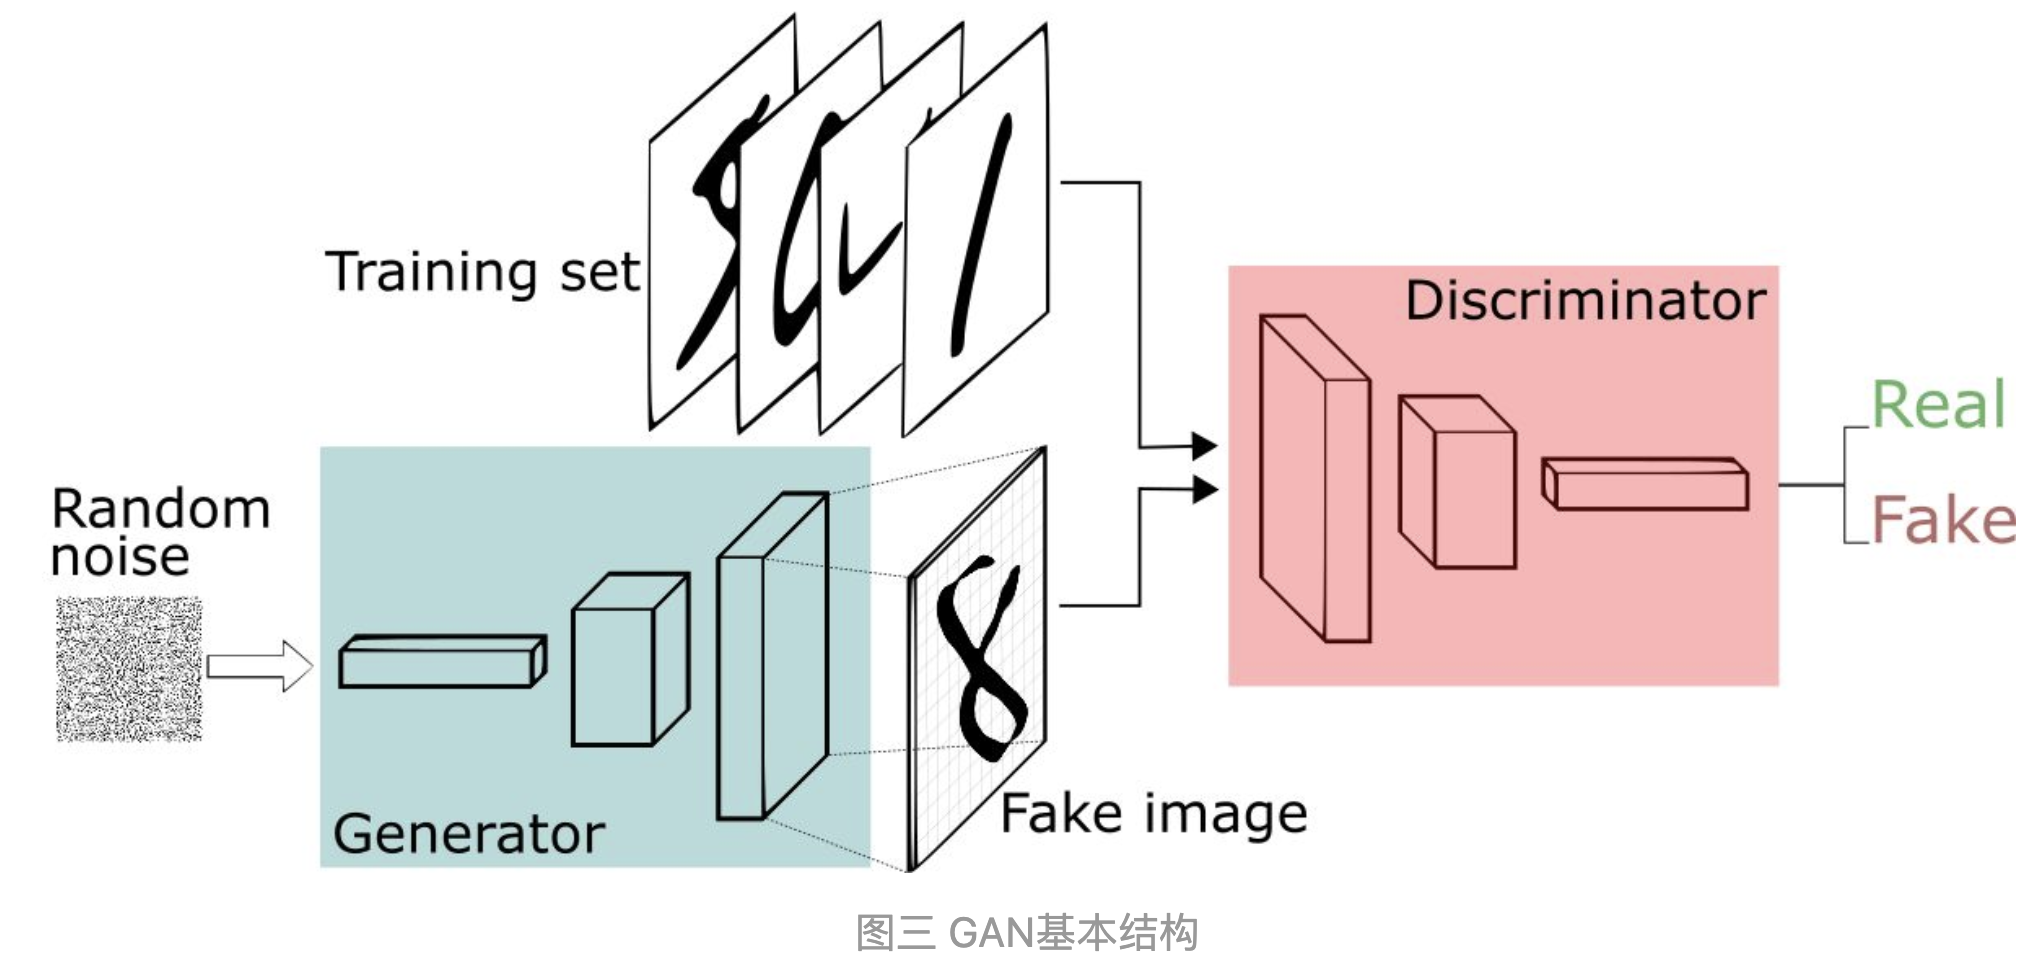
\includegraphics[width=1\textwidth]{fig/GAN_Basic_Structure.png}
\end{figure}

我们现在拥有大量的手写数字的数据集,我们希望通过GAN生成一些能够以假乱真的手写字图片。主要由如下两个部分组成:
\begin{enumerate}
\setlength{\itemsep}{0pt}
\setlength{\parsep}{0pt}
\setlength{\parskip}{0pt}
    \item 定义一个模型来作为生成器(图三中蓝色部分Generator),能够输入一个向量,输出手写数字大小的像素图像。
    \item 定义一个分类器来作为判别器(图三中红色部分Discriminator)用来判别图片是真的还是假的(或者说是来自数据集中的还是生成器中生成的),输入为手写图片,输出为判别图片的标签。
\end{enumerate}

\subsection{GAN的训练方式}
前面已经定义了一个生成器(Generator)来生成手写数字,一个判别器(Discriminator)来判别手写数字是否是真实的,和一些真实的手写数字数据集。那么我们怎样来进行训练呢?

\subsubsection{关于生成器}
对于生成器,输入需要一个 $n$ 维度向量,输出为图片像素大小的图片。因而首先我们需要得到输入的向量。

Tips: 这里的生成器可以是任意可以输出图片的模型,比如最简单的全连接神经网络,又或者是反卷积网络等。

这里输入的向量我们将其视为携带输出的某些信息,比如说手写数字为数字几,手写的潦草程度等等。由于这里我们对于输出数字的具体信息不做要求,只要求其能够最大程度与真实手写数字相似(能骗过判别器)即可。所以我们使用随机生成的向量来作为输入即可,这里面的随机输入最好是满足常见分布比如均值分布,高斯分布等。

Tips: 假如我们后面需要获得具体的输出数字等信息的时候,我们可以对输入向量产生的输出进行分析,获取到哪些维度是用于控制数字编号等信息的即可以得到具体的输出。而在训练之前往往不会去规定它。

\subsubsection{关于判别器}
对于判别器不用多说,往往是常见的判别器,输入为图片,输出为图片的真伪标签。

Tips: 同理,判别器与生成器一样,可以是任意的判别器模型,比如全连接网络,或者是包含卷积的网络等等。

小结:判别器网络是一个标准的能够分类图片的卷积网络,是一个二分类器标记图片的真假。生成器网络是一个反卷积网络,在某种意义上讲,标准卷积分类器对图片进行下采样并切生成一个排律,生成器会生成随机噪声向量并将其上采样成一张图片。判别器网络是通过像maxpooling下采样丢弃数据,生成器则是生成新数据。

\subsubsection{如何训练}
上面进一步说明了生成器和判别器,接下来说明如何进行训练。

基本流程如下:
\begin{itemize}
\setlength{\itemsep}{0pt}
\setlength{\parsep}{0pt}
\setlength{\parskip}{0pt}
    \item 初始化判别器D的参数 $\theta_d$ 和生成器G的参数 $\theta_g$。
    \item 从真实样本中采样$m$个样本$\{x^1, x^2, \cdots, x^m\}$;从先验分布噪声中采样$m$个噪声样本  $\{z^1, z^2, \cdots, z^m\}$ ,并通过生成器获取个 $m$ 生成样本 $\{\tilde{x}^1 , \tilde{x}^2, \cdots, \tilde{x}^m\}$。固定生成器G,训练判别器D尽可能好地准确判别真实样本和生成样本,尽可能大地区分正确样本和生成的样本。
	\item 循环$k$次更新判别器之后,使用较小的学习率来更新一次生成器的参数,训练生成器使其尽可能能够减小生成样本与真实样本之间的差距,也相当于尽量使得判别器判别错误。
	\item 多次更新迭代之后,最终理想情况是使得判别器判别不出样本来自于生成器的输出还是真实的输出。亦即最终样本判别概率均为0.5。
\end{itemize}

\begin{framed}
之所以要训练$k$次判别器,再训练生成器,是因为要先拥有一个好的判别器,使得能够教好地区分出真实样本和生成样本之后,才好更为准确地对生成器进行更新。更直观的理解可以参考下图:
\begin{figure}[H]
    \centering
    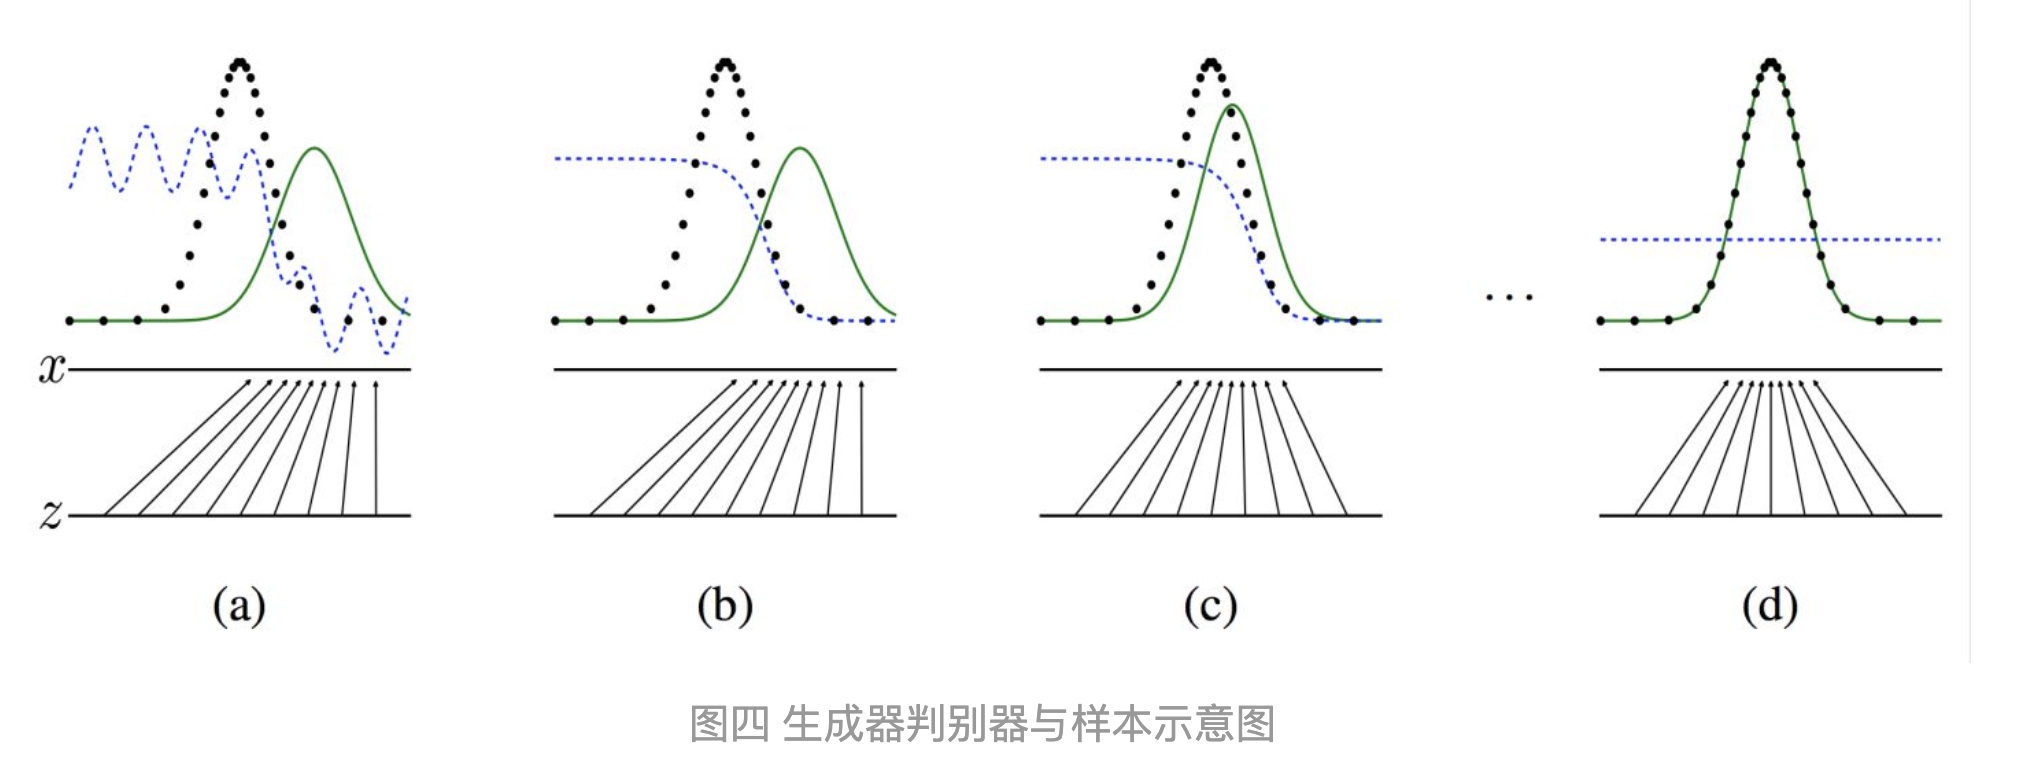
\includegraphics[width=1\textwidth]{fig/GAN_Generator_Discriminator_Example.png}
\end{figure}

注:图中的黑色虚线表示真实的样本的分布情况,蓝色虚线表示判别器判别概率的分布情况,绿色实线表示生成样本的分布。 $Z$ 表示噪声, $Z$ 到 $x$ 表示通过生成器之后的分布的映射情况。

我们的目标是使用生成样本分布(绿色实线)去拟合真实的样本分布(黑色虚线),来达到生成以假乱真样本的目的。

可以看到在(a)状态处于最初始的状态的时候,生成器生成的分布和真实分布区别较大,并且判别器判别出样本的概率不是很稳定,因此会先训练判别器来更好地分辨样本。

通过多次训练判别器来达到(b)样本状态,此时判别样本区分得非常显著和良好。然后再对生成器进行训练。

训练生成器之后达到(c)样本状态,此时生成器分布相比之前,逼近了真实样本分布。

经过多次反复训练迭代之后,最终希望能够达到(d)状态,生成样本分布拟合于真实样本分布,并且判别器分辨不出样本是生成的还是真实的(判别概率均为0.5)。也就是说我们这个时候就可以生成出非常真实的样本啦,目的达到。
\end{framed}



\subsection{训练相关理论基础}
前面用了大白话来说明了训练的大致流程,下面会从交叉熵开始说起,一步步说明损失函数的相关理论,尤其是论文中包含min,max的公式如下面的形式:
\begin{figure}[H]
    \centering
    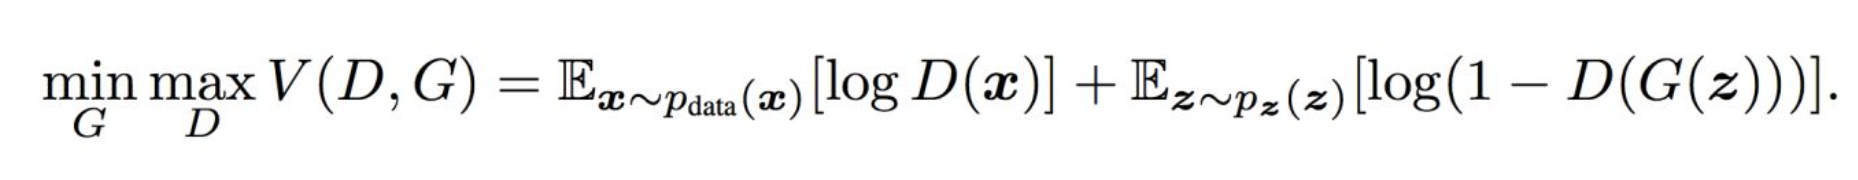
\includegraphics[width=1\textwidth]{fig/GAN_Eq_Minmax.png}
\end{figure}

\subsubsection{交叉熵}
判别器在这里是一种分类器,用于区分样本的真伪,因此我们常常使用交叉熵(cross entropy)来进行判别分布的相似性,交叉熵公式如下所示:
$$
H(p,q) = -\sum_{i}p_i\log q_i
$$

公式中 $p_i$ 和 $q_i$ 为真实的样本分布和生成器的生成分布。

在当前模型的情况下,判别器为一个二分类问题,因此可以对基本交叉熵进行更具体地展开为二分类交叉熵,如下所示:
$$
H((x_1, y_1), D) = -y_1\log D(x_1) - (1-y_1)\log(1-D(x_1))
$$

其中,假定 $y_1$ 为正确样本分布,那么对应的 $(1-y_1)$ 就是错误样本的分布。 $D$ 表示判别器,则 $D(x_1)$ 表示判别样本为正确的概率,$(1-D(x_1)$则对应着判别为错误样本的概率。

将上式推广到$N$个样本后,将$N$个样本相加得到对应的公式如下:
$$
H((x_i, y_i)^N_{i=1}, D) = -\sum_{i=1}^N\Big(-y_1\log D(x_1)\Big)- \sum_{i=1}^N\Big((1-y_1)\log(1-D(x_1))\Big)
$$

\subsubsection{对应到 GAN}
对于GAN中的样本点 $x_i$ ,对应于两个出处:要么来自于真实样本,要么来自于生成器生成的样本$\tilde{x} \sim G(z)$ ( 这里的 $z$ 是服从于投到生成器中噪声的分布)。

其中,对于来自于真实的样本,我们要判别为正确的分布 $y_i$ 。来自于生成的样本我们要判别其为错误分布$(1-y_i)$。将上面式子进一步使用概率分布的期望形式写出(为了表达无限的样本情况,相当于无限样本求和情况),并且让$y_i$为 1/2 且使用 $G(z)$表示生成样本可以得到如下公式:

$$
H((x_i, y_i)^\infty_{i=1}, D) = -\frac{1}{2}\mathbb{E}_{x\sim p_{data}}\Big[\log D(x)\Big] - \frac{1}{2}\mathbb{E}_z\Big[\log(1-D(G(z)))\Big]
$$

\subsubsection{GAN中的 min 和 max}
现在我们再回过头来对比原本的的 $\min\limits_G \max\limits_D$ 公式,发现他们是不是其实就是同一个东西呢:
\begin{figure}[H]
    \centering
    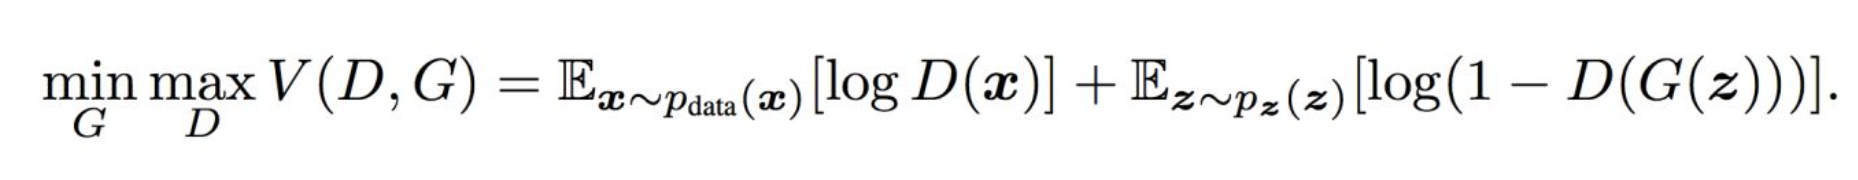
\includegraphics[width=1\textwidth]{fig/GAN_Eq_Minmax.png}
\end{figure}

\begin{itemize}
\setlength{\itemsep}{0pt}
\setlength{\parsep}{0pt}
\setlength{\parskip}{0pt}
    \item 这里的 $V(G,D)$ 相当于表示真实样本和生成样本的差异程度。
    \item 先看 $\max\limits_D$。这里的意思是固定生成器G,尽可能地让判别器能够最大化地判别出样本来自于真实数据还是生成的数据。
    \item 再将后面部分看成一个整体令 $L = \max\limits_D V(D,G)$ ,看 $\min\limits_G L$,这里是在固定判别器D的条件下得到生成器G,这个G要求能够最小化真实样本与生成样本的差异。
    \item 通过上述min max的博弈过程,理想情况下会收敛于生成分布拟合于真实分布。
\end{itemize}

\subsection{D 的训练过程推导}
当生成器G固定时,我们可以对V(D,G)求导,求出最优判别器 $D^*(x)$:
$$
D^*(x) = \frac{p_{data}(x)}{p_g(x) + p_{data}(x)}
$$

把最优判别器代入上述目标函数,可以进一步求出在最优判别器下,生成器的目标函数等价于优化 $p_{data}(x)$, $p_g(x)$ 的JS散度(JSD, Jenson Shannon Divergence)。

可以证明,当G,D二者的capacity足够时,模型会收敛,二者将达到纳什均衡。此时,$p_{data}(x) = p_g(x)$ ,判别器不论是对于 $p_{data}(x) $ 还是  $p_g(x)$ 中采样的样本,其预测概率均为$\frac{1}{2}$,即生成样本与真实样本达到了难以区分的地步。

\subsection{目标函数}
前面我们提到了GAN的目标函数是最小化两个分布的JS散度。实际上,衡量两个分布距离的方式有很多种,JS散度只是其中一种。如果我们定义不同的距离度量方式,就可以得到不同的目标函数。许多对GAN训练稳定性的改进,比如EBGAN,LSGAN等都是定义了不同的分布之间距离度量方式。

\subsubsection{f-divergence}
f-divergence使用下面公式来定义两个分布之间的距离:
$$
D_f(p_{data}||p_g) =  \int_x p_g(x) f\Big(\frac{p_{data}(x)}{p_g(x)}\Big)dx
$$

值得注意的是,散度这种度量方式不具备对称性,即 $D_f(p_{data}||p_g)$ 和$D_f(p_g||p_{data}||)$不相等(严格来说,距离度量方式必须具备对称性,所以散度不是一种距离度量方式,不过此处不去刻意关注这一点,直接把散度也作为一种距离度量方式,下文也是如此)。



上述公式中 $f$ 为凸函数,且 $f(1) = 0$。采用不同的 $f$ 函数(Generator),可以得到不同的优化目标。具体如下:
\begin{figure}[H]
    \centering
    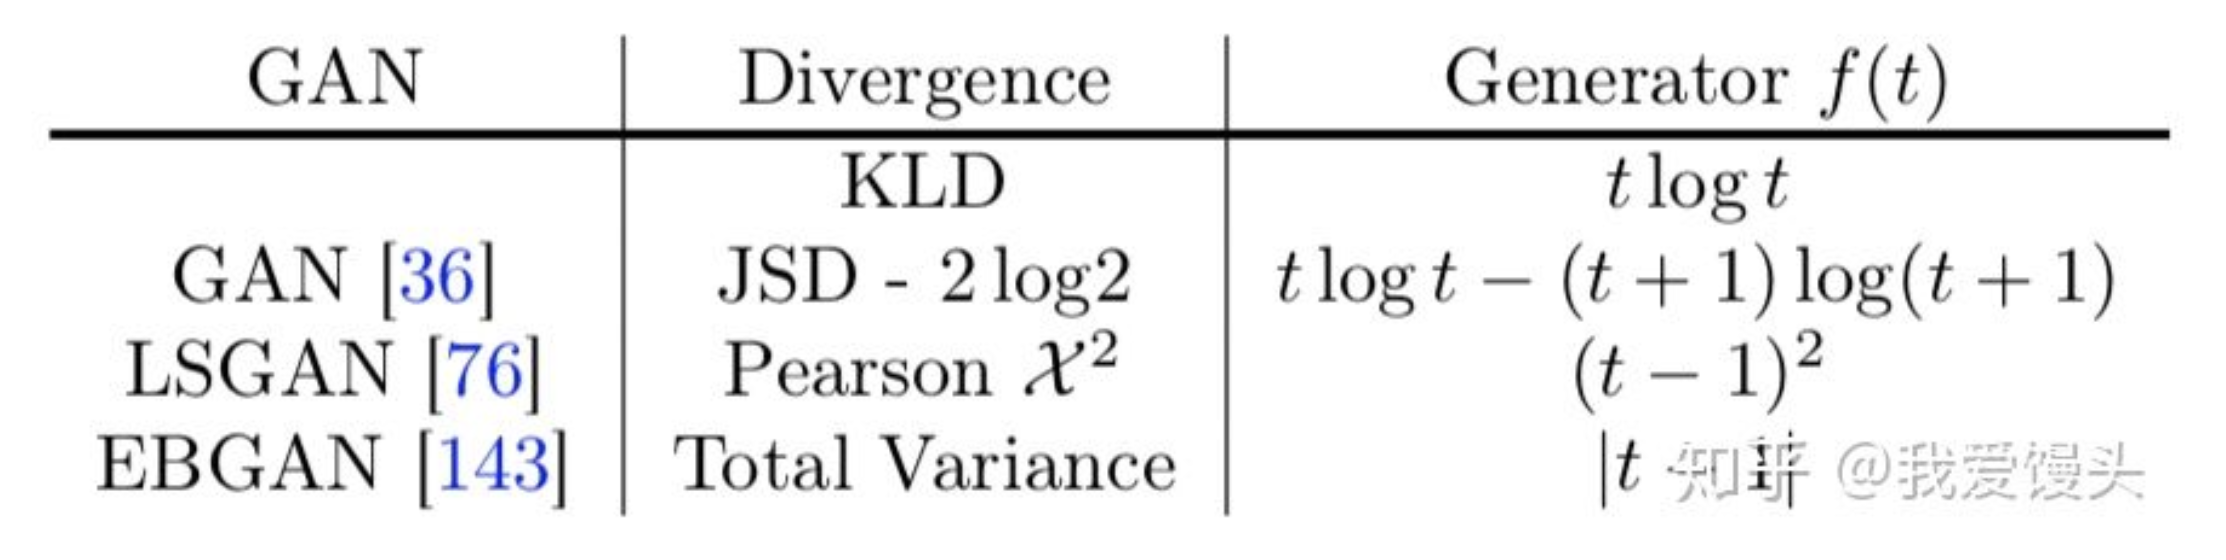
\includegraphics[width=.8\textwidth]{fig/GAN_Diff_F_Divergence.png}
\end{figure}


\subsection{GANs、自编码器 和 VAEs}
将GANs和其他神经网络做比较是非常有用的,比如自编码器和变分自编码器(VAEs)。

自编码器对输入数据编码成向量,它们创造对原始数据的隐藏、或是压缩表示。它们对降低维数很有用,也就是说,用作隐藏表示的向量讲原始数据压缩成更少量的主要维度。自编码器能够和解码器共同存在,解码器允许你对基于隐藏表示的输入数据进行重构,就像需要用受限制玻尔兹曼机一样。
\begin{figure}[H]
    \centering
    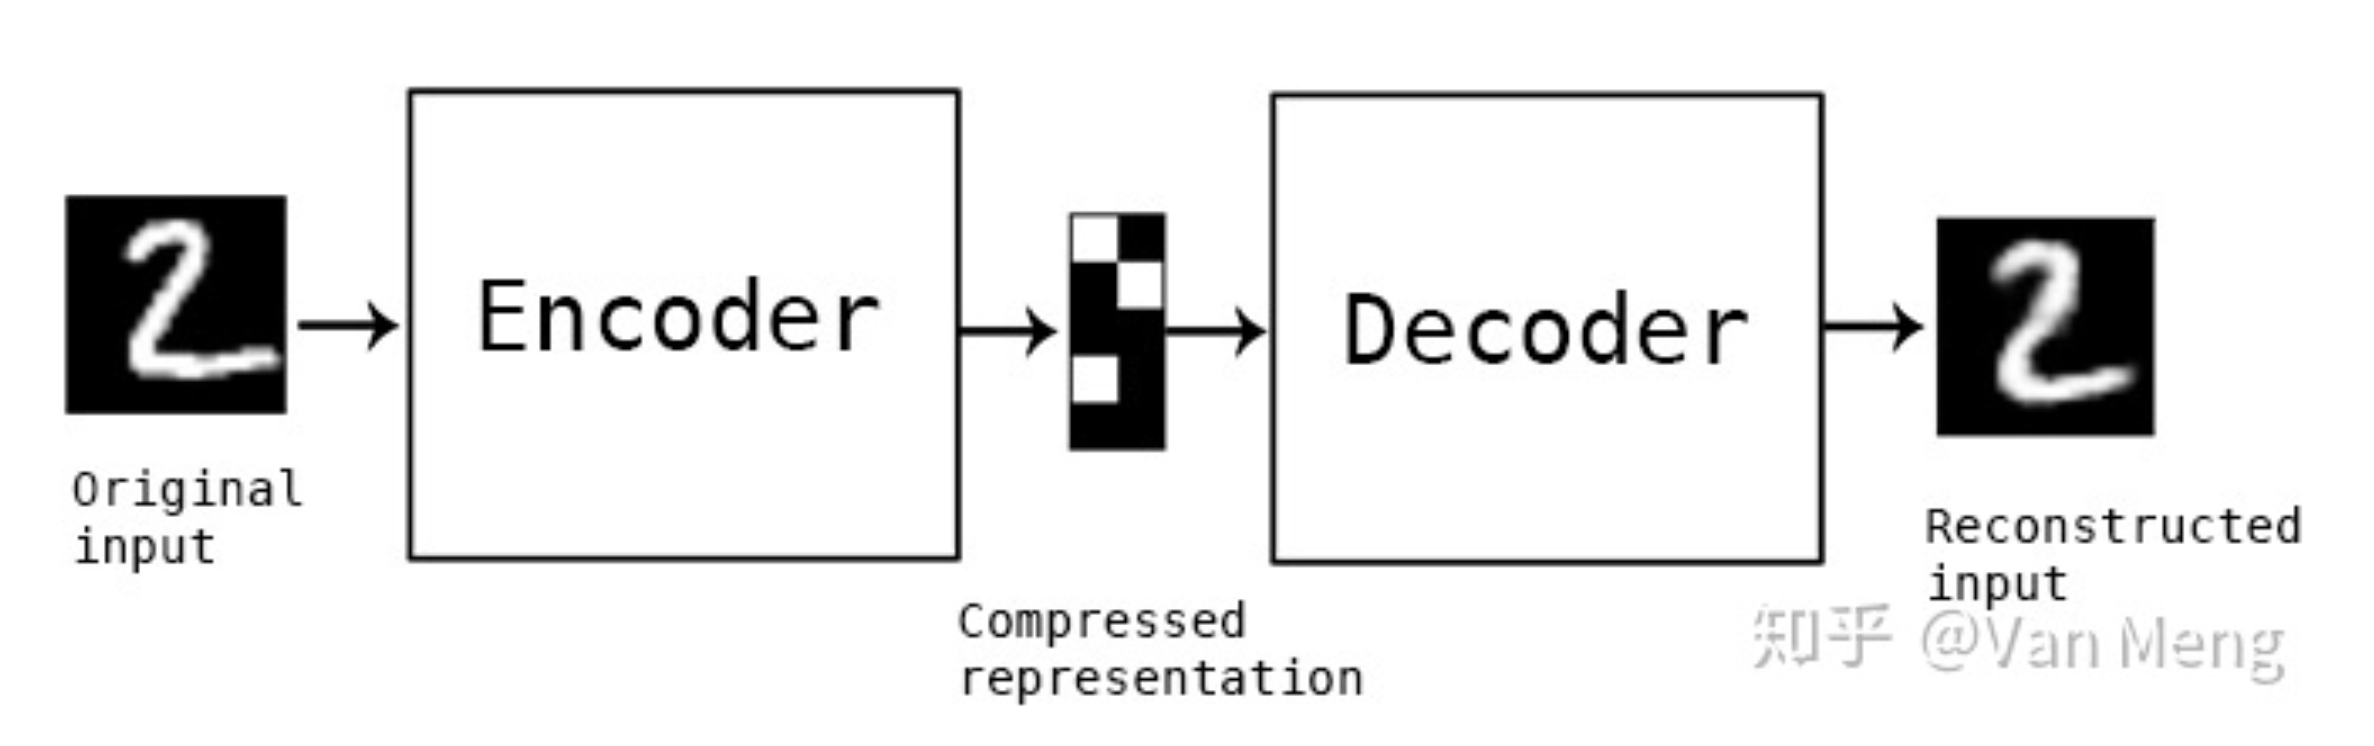
\includegraphics[width=1\textwidth]{fig/GAN_AutoEncoder.png}
\end{figure}

变分自编码器是一种生成算法,它对输入数据的编码添加了额外的限制,即隐藏表示被标准化。变分自编码器能够像自编码器一样压缩数据,也能像GAN一样合成数据。当然,GAN生成的数据是精细的,VAEs生成的数据更加模糊。Deeplearning4j的例子包含 自编码器和变分自编码器.

你可以将生成算法分为以下三类:
\begin{itemize}
\setlength{\itemsep}{0pt}
\setlength{\parsep}{0pt}
\setlength{\parskip}{0pt}
    \item 给定标签,预测相关特征(朴素贝叶斯)
    \item 给定隐藏表示,预测相关特征(VAE,GAN)
    \item 给定特征,预测其他(修复、插补)
\end{itemize}

\section{扩展阅读}
入门材料:A Beginner's Guide to Generative Adversarial Networks (GANs)


%\printbibliography
\bibliography{../ref}
\bibliographystyle{IEEEtran}
\end{document}